\documentclass[10pt,a4paper]{article}
\usepackage[utf8]{inputenc}
\usepackage{amsmath}
\usepackage{amsfonts}
\usepackage{amssymb}
\usepackage{cite}
\usepackage{hyperref}
\usepackage{graphicx}


\begin{document}

\title{Product Vision\\
	\begin{small}
	The why, who and what
	\end{small}
}
% Question: should this be our names or organization name?
\author{MoodCat.me}
\maketitle

\section{Why should we build MoodCat?}
Various competitors provide a system that can offer users popular songs or songs that are similar to songs the user already listened to.
These recommendations mostly consist of songs that are popular or users with simmilar preferences listened to.
This leaves a tremendous chunk of music produced by a lot of artists undiscovered.

Secondly, most music platforms do not offer user interaction.
Some competitors offer users rooms to socialize while experiencing songs.
An example is Plug DJ \cite{PlugDJ} where users can create a room and listeners can suggest Youtube-songs\cite{Youtube} for the playlist.
Such a playlist has to be maintained in order to keep running and therefore does not suit the listeners that want to listen on their own.
Furthermore, it has to be moderated to prevent unwanted suggestions that might not be interesting for the listeners.

\bigskip 

Users want to discover music and have social interaction.
MoodCat allows users (and friends!) to unite in rooms, and listen to and discuss music together.
Hereby we apply a successful feature from the live video/gaming streaming industry (for example TwitchTV \cite{Twitch}) to the music industry.
Music rooms never fall silent, instead they are continuously filled with relevant music that fits the mood of the listeners in the room.

\section{What is the target audience of MoodCat?}
Our target audience consists of (but not limiting to) the following persons:

\begin{enumerate}
\item Everyone who wants to listen to music without the hassle of searching suitable songs for their current mood/preferences.

\item Everyone who wants to discover and listen to songs they haven't heard yet.

\item Everyone who wants to listen to and experience songs and share this experience with fellow listeners in the same online room.

\item Everyone who wants to listen at any time on the day, no matter how many users are currently online.
\end{enumerate}

\section{What are the selling points of MoodCat?}
MoodCat has several selling points that would make it unique in the current music market.

\begin{enumerate}
\item MoodCat is self-maintaining, which makes it possible to handle audience sizes from one to one thousand.
This makes it possible to use the system no matter how many other users are currently online.

\item MoodCat offers users both to experience solely or communicate with fellow music listeners.

\item The system already works without this user input as specific interpretation of audio features allow us to find similar songs.
The system is able to offer relevant songs using the specified current mood of the user.

\item With MoodCat unknown/lesser known artists have equal chances to let their songs be played.
This is a result of the system choosing songs based on features and is therefore unbiased regarding play counts.

\item MoodCat can determine mood trends of a long-term user and can adjust the room-ordering mechanism accordingly.
Therefore long-term users are served more suitable rooms which increases their overall satisfaction.

\item MoodCat can suggest users who are repeatedly not satisfied with the songs played in a room, a different and more suitable room.
\end{enumerate}

\section{Which components should MoodCat have?}
MoodCat will be developed as three seperate componentents: the frontend, the backend and a special music matching algorithm.

\begin{enumerate}
\item The frontend will be the visible part for the listener.
After logging in to our services, the user will be able to select his mood and based on that MoodCat will provide several music listening rooms.
In these rooms the user can interact with other listeners through the chat while listening to the music.

\item The backend keeps track of which rooms are active and what song is currently played in the room.
Furthermore, the backend is responsible for transmitting the chat messages between the users in the room.

\item The music matching algorithm is used to compare and match moods of songs and chatrooms.
It has two roles: list the room suggestions for a user and provide the next song to be played for a room.
\end{enumerate}

\newpage

\subsection{Frontend}

The MoodCat frontend will be web-based. This allows us to support all modern devices which enables a large target audience. We will develop the frontend using modern techniques as HTML5, CSS3 and AngularJS. Users can login using their Soundcloud account. This allows us to integrate with the Soundcloud platform and prevents having to register for our services first.

\subsection{Backend}

The MoodCat backend will be a RESTful API written in Java using JAX-RS. It will be backed by a relational (PostgreSQL) database. The backend connects the frontend to the music matching algorithm.

\subsection{Music matching algorithm}

During our research about mapping music to emotions/moods, we discovered the valence/arousal graph (see figure \ref{fig:avgraph}).
This graph appears to be used in a lot of scientifical projects.

\begin{figure}[h]
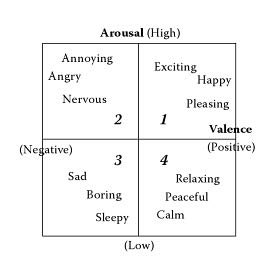
\includegraphics[scale=0.75]{avgraph.jpg}
\caption{The valance/arousal graph \cite{Book}}
\label{fig:avgraph}

\end{figure}

Arousal and valence are physiological terms.
Arousal means how calm or excited you are.
Valence is the amount of attraction you have towards a certain event.

In order to use arousal and valence, we have to express them in terms of music features.
For valence we can use harmony \cite{PresentationMER},mode  \cite{PresentationMER} and tonality  \cite{PresentationMER}.
For arousal we can use pitch \cite{PresentationMER} ,timbre \cite{PresentationMER}, tempo \cite{PresentationMER} and loudness \cite{PaperME}.

\newpage

The data of EEMCS does not explicitly provide the above features. However, we can extract them from the low-level features the data does provide.

The low-level features we can use for valence:
\begin{enumerate}
\item For harmony we can use the dissonance of a song.
\item To determine the key of a song, we can use the mode.
\item Finally the tonal provides the information to obtain the tonality.
\end{enumerate}
The low-level features we can use for arousal:
\begin{enumerate}
\item BMP gives us insight of the tempo of a song
\item Loudness can be directly retrieved from the loudness feature.
\end{enumerate}

The timbre of a song is a seperate research field and is too difficult to integrate into our system.

Even so we couldn't find a low level feature in the dataset that describes the pitch of a song.
We did find 'pitch salience', however this only describes whether a song is pitched or not.
This does not give any information on how low or high the pitch of the song is.

%
% BIBLIOGRAPHY
%

\begin{thebibliography}{10}
\bibitem{PlugDJ} http://www.plug.dj
\bibitem{Youtube} http://www.youtube.com
\bibitem{Twitch} http://www.twitch.tv
\bibitem{PresentationMER} Chen, h. H. (2013). Music Emotion Recognition [pdf]. http://www2.ensc.sfu.ca/~ljilja/cnl/guests/Music.pdf
\bibitem{PaperME} http://cisaweb.unige.ch/drupal/system/files/biblio/emo-11-4-921.pdf (p. 924)
\bibitem{Book} Chang,Y. and Chen,H.H. (2011) Music Emotion Recognition. Boca raton, State: CRC Press %https://www.google.com.tr/books?hl=en&lr=&id=qnjRBQAAQBAJ&oi=fnd&pg=PP1&dq=music+mood+recognition&ots=0HTz4SBc2J&sig=9VEW6tZRGeOwGnuhTRYbO453_2U&redir_esc=y#v=onepage&q=music%20mood%20recognition&f=false

\end{thebibliography}

\end{document}